
%(BEGIN_QUESTION)
% Copyright 2008, Tony R. Kuphaldt, released under the Creative Commons Attribution License (v 1.0)
% This means you may do almost anything with this work of mine, so long as you give me proper credit

{\it Derivative} control action is especially useful in processes characterized by slow lag times, especially when the process has a natural tendency to ``overshoot'' the setpoint due to multiple lags.  The purpose of derivative mode control is to make decisions based on how {\it quickly} the process variable changes over time, taking action in the present to avoid setpoint overshoot in the future.

However, derivative mode control cannot be used in processes where the PV signal is tainted with {\it noise}, as is the case in this trend:

$$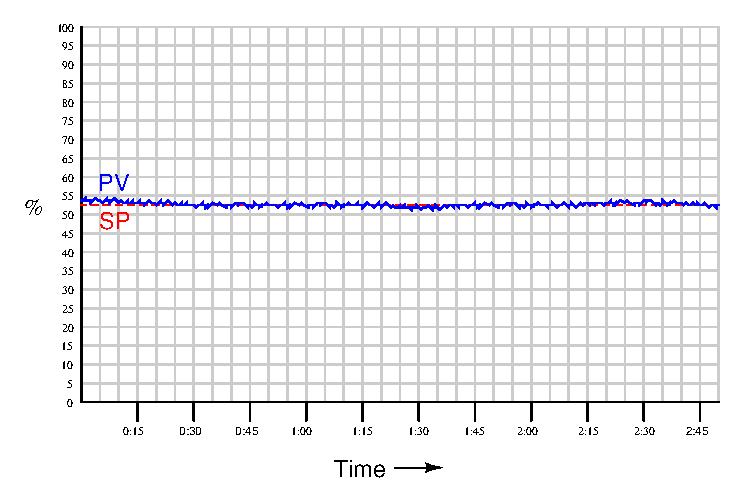
\includegraphics[width=15.5cm]{i01671x01.eps}$$

It does not matter how well-suited the process may be for derivative control in any other regard, so long as the noise is there.  Noise and derivative control are simply incompatible -- explain why.

\vskip 10pt

Also, identify whether or not {\it integral} mode control is affected by noise in the PV signal, and explain your answer.

\vskip 20pt \vbox{\hrule \hbox{\strut \vrule{} {\bf Suggestions for Socratic discussion} \vrule} \hrule}

\begin{itemize}
\item{} Observing the trend graph shown here, can we tell whether this controller is in manual mode or automatic mode?  If so, identify its operating mode.
\item{} Observing the trend graph shown here, can we tell whether this controller is direct-acting or reverse-acting?  If so, identify its direction of action.
\item{} Observing the trend graph shown here, can we tell anything about the P, I, and/or D settings of this controller?  If so, identify what its dominant control action is (P, I, or D).
\end{itemize}

\underbar{file i01671}
%(END_QUESTION)





%(BEGIN_ANSWER)


%(END_ANSWER)





%(BEGIN_NOTES)

Derivative ``sees'' the noise signal as having extremely large rates-of-change over time, and reacts accordingly.  Practically any amount of derivative programmed into the controller seeing this noisy PV signal will cause the controller's output to wildly fluctuate.

\vskip 10pt

Integral, on the other hand, practically ignores noise.  Even when the PV noise is severe, and the integral time constant very short (i.e. aggressive integral action), integral-mode control does not take any measurable action on the noise signal.  Integral action ``sees'' the above-setpoint and below-setpoint noise spikes as nearly equal and opposite errors over time.  Therefore, their net error-time product contribution to the integral control action will be practically zero.

%INDEX% Control, derivative: noisy process signal
%INDEX% Control, integral: noisy process signal
%INDEX% Control, PID tuning: inappropriate applications for derivative control action

%(END_NOTES)


